% !TeX root = ../alm20171206.tex
% !TeX encoding = UTF-8
% !TeX spellcheck = en_US


%% == LaTeX ============================================================= %%
%% https://en.wikibooks.org/wiki/LaTeX
%% ====================================================================== %%


%% -- 2.4 Colors -------------------------------------------------------- %%
%% https://en.wikibooks.org/wiki/LaTeX/Colors
% \usepackage[usenames,dvipsnames,svgnames,table]{xcolor}
% % !TeX encoding = UTF-8
% !TeX spellcheck = en_US

%% https://en.wikibooks.org/wiki/LaTeX/Colors

%% color definitions

% \colorlet{col:a}{Fuchsia}
% \colorlet{col:b}{Blue}
\colorlet{colG}{Gray}
\colorlet{colO}{Orange}
\colorlet{colHi}{Green}
\colorlet{colLo}{Red}
\colorlet{colNa}{Gray}
\colorlet{colN}{Blue}
\colorlet{colEm}{RoyalBlue}
\colorlet{colMAXIMAL}{Violet}
\colorlet{colSTRICTLY}{RoyalBlue}

%% PAINT IT BLACK =========
% \colorlet{col:a}{black}
% \colorlet{col:b}{black}
% \colorlet{colG}{black}
% \colorlet{colO}{black}
% \colorlet{colHi}{black}
% \colorlet{colLo}{black}
% \colorlet{colNa}{black}
% \colorlet{colN}{black}
% \colorlet{colEm}{black}
% \colorlet{colMAXIMAL}{black}
% \colorlet{colSTRICTLY}{black}

%\newcommand{\colA}{\color{col:a}}	% example a
%\newcommand{\colB}{\color{col:b}}	% example b
\newcommand{\colG}{\color{colG}}	% neutral
\newcommand{\colO}{\color{colO}}	% old
\newcommand{\colN}{\color{colN}}	% new
\newcommand{\colHi}{\color{colHi}}	% hi, true
\newcommand{\colLo}{\color{colLo}}	% lo, false
\newcommand{\colNA}{\color{colNa}}	% not available
\newcommand{\colEm}{\color{colEm}}

%\newcommand{\colMax}{\color{colMax}}	% maximal
%\newcommand{\colSmx}{\color{colSmx}}	% strictly maximal

%\newcommand{\MYa}{\color{Fuchsia}}
%\newcommand{\MYb}{\color{Blue}}
%\newcommand{\MYg}{\color{Gray}}
%\newcommand{\MYo}{\color{Orange}}
%
%\newcommand{\MYhi}{\color{Green}}
%\newcommand{\MYlo}{\color{Red}}
%\newcommand{\MYna}{\color{Gray}}
%
%\newcommand{\MYA}[1]{{\MYa#1}}
%\newcommand{\MYB}[1]{{\MYb#1}}
%\newcommand{\MYG}[1]{{\MYg#1}}
%\newcommand{\MYO}[1]{{\MYo#1}}
%
%\newcommand{\MYHI}[1]{{\MYhi#1}}
%\newcommand{\MYLO}[1]{{\MYlo#1}}
%\newcommand{\MYNA}[1]{{\MYna#1}}
%
%\newcommand{\MYS}[1]{{\color{Violet}#1}}
%\newcommand{\MYM}[1]{{\color{RoyalBlue}#1}}
%
%\newcommand{\mLightning}{{\text{\Lightning}}}

%% ---------------------------------------------------------------------- %%


%% -- 2.8 Internationalization ------------------------------------------ %%
%% https://en.wikibooks.org/wiki/LaTeX/Internationalization
\usepackage[utf8x]{inputenc} 		% input
\usepackage[LGR,T1]{fontenc}	 	% output (PDF)
\usepackage[english]{babel}			% language

%% ---------------------------------------------------------------------- %%


%% -- 2.10 Tables ------------------------------------------------------- %%
% https://en.wikibooks.org/wiki/LaTeX/Tables
%% ---------------------------------------------------------------------- %%


%% -- 2.16-17 Hyperlinks ------------------------------------------------ %%
% https://en.wikibooks.org/wiki/LaTeX/Hyperlinks
% https://en.wikibooks.org/wiki/LaTeX/Labels_and_Cross-referencing
\usepackage{hyperref}
% %\usepackage[xindy,toc]{glossaries}
% \usepackage[toc]{glossaries}
% \usepackage[]{index}
% %% ---------------------------------------------------------------------- %%


%% -- 4.1-3 Mathematics ------------------------------------------------- %%
% https://en.wikibooks.org/wiki/LaTeX/Mathematics
% https://en.wikibooks.org/wiki/LaTeX/Advanced_Mathematics
\usepackage{amsmath}
\usepackage{mathtools}
\usepackage{amssymb}

% https://en.wikibooks.org/wiki/LaTeX/Theorems
\usepackage{amsthm}
\usepackage{proof}
% \usepackage{bussproofs}
% \usepackage{marvosym}

% \usepackage{multirow}
% \usepackage[makeroom]{cancel} % \(b|x)cancel(to{}){}
% \usepackage{soul}
% \usepackage{pdfcomment}


%% ---------------------------------------------------------------------- %%


\usepackage{varioref}


%\usepackage{calc}
%\usepackage{geometry}

%% -- 4.5 Algorithms ---------------------------------------------------- %%
% https://en.wikibooks.org/wiki/LaTeX/Algorithms
%% ---------------------------------------------------------------------- %%


%% -- 4.6 Listings ------------------------------------------------------ %%
% https://en.wikibooks.org/wiki/LaTeX/Source_Code_Listings
% \usepackage{listings}
% % !TeX encoding = UTF-8
% !TeX spellcheck = en_US

\lstdefinelanguage{smtlib}{
	comment={[l];},
	keywords={assert,xor, or, and},
	otherkeywords={declare-fun, set-logic},
	emph={Int,QF_LIA},
}

\lstdefinelanguage{Yices}{
	language = C,
	morekeywords={},
%	comment={[l];},
%	keywords={assert,xor, or, and},
	keywords=[2]{type_t, uint32_t, term_t},
%	emph={Int,QF_LIA},
%	otherkeywords={yices_bool_type}
}

\lstdefinelanguage{flea}{
	language = C,
%	morekeywords={},	
	%	comment={[l];},
	%	keywords={assert,xor, or, and}, 	% 
	keywords=[2]{func, var, let, protocol, associatedtype, extension},	% Swift Keywords
	keywords=[3]{String, UInt32},					% Swift data types
	keywords=[4]{type_t, uint32_t, term_t,},		% yices data types
	%%% begin yices API keywords %%%
	keywords=[5]{yices_get_type_by_name, yices_new_uninterpreted_term, yices_new_uninterpreted_type}				
	%%% end yices API keywords %%%
	%	emph={Int,QF_LIA},
	%	otherkeywords={yices_bool_type}
}

\lstset {
	backgroundcolor=\color{white},     	% choose the background color; you must add \usepackage{color} or \usepackage{xcolor}
	basicstyle=\ttfamily\footnotesize, 	% the size of the fonts that are used for the code
	breakatwhitespace=false,         	% sets if automatic breaks should only happen at whitespace
	breaklines=true,                 	% sets automatic line breaking
	caption=\lstname,
	captionpos=b,                    	% sets the caption-position to bottom
	commentstyle=\color{gray},    		% comment style
	deletekeywords={...},            	% if you want to delete keywords from the given language
	emphstyle=\color{orange},
	escapeinside={\%*}{*)},         % if you want to add LaTeX within your code
	extendedchars=true,             % lets you use non-ASCII characters; for 8-bits encodings only, does not work with UTF-8
	frame=none,		% frame=single, % adds a frame around the code
	keepspaces=true,                % keeps spaces in text, useful for keeping indentation of code (possibly needs columns=flexible)
	keywordstyle=\color{OliveGreen},      % keyword style
	keywordstyle=[2]\color{Fuchsia},
	keywordstyle=[3]\color{RedViolet},
	keywordstyle=[4]\color{RoyalBlue},	% yices data types
	keywordstyle=[5]\color{NavyBlue},	% yices api
	% language=smtlib,	%Octave,    % the language of the code
	% literate={;},
	% otherkeywords={declare-fun,set-logic,assert,xor,or,and},            % if you want to add more keywords to the set
	%morecomment=[l]{;}				% line comment
	numbers=left,                   % where to put the line-numbers; possible values are (none, left, right)
	numbersep=5pt,                  % how far the line-numbers are from the code
	numberstyle=\tiny\color{gray}, 	% the style that is used for the line-numbers
	rulecolor=\color{black},        % if not set, the frame-color may be changed on line-breaks within not-black text (e.g. comments (green here))
	showspaces=false,               % show spaces everywhere adding particular underscores; it overrides 'showstringspaces'
	showstringspaces=false,         % underline spaces within strings only
	showtabs=false,                 % show tabs within strings adding particular underscores
	stepnumber=1,                   % the step between two line-numbers. If it's 1, each line will be numbered
	stringstyle=\color{orange},     % string literal style
	tabsize=2,	                   	% sets default tabsize to 2 spaces
%	title=\lstname,                  % show the filename of files included with \lstinputlisting; also try caption instead of title,
	mathescape=true
}
	% definitions
% %% ---------------------------------------------------------------------- %%


% %% -- Graphics ---------------------------------------------------------- %%
% % https://en.wikibooks.org/wiki/LaTeX/PGF/TikZ
% \usepackage{tikz}
% \documentclass{clseminar}

    \usepackage{tikz}
    \usepackage{soul}

    % \documentclass{clseminar}

    \usepackage{tikz}
    \usepackage{soul}

    % \documentclass{clseminar}

    \usepackage{tikz}
    \usepackage{soul}

    % \input{../PREAMBLE/Drawings}

\begin{document}

\begin{figure}
    \begin{center}
\input{../DRAWINGS/ProperOrder}
\caption{Proper orders on terms}
    \end{center}
\end{figure}

\begin{figure}
    \begin{center}
\input{../DRAWINGS/PartialOrder}
\caption{Equivalence relation vs.~partial order}
\end{center}
\end{figure}

\end{document}

\begin{document}

\begin{figure}
    \begin{center}
\begin{tikzpicture}
    \node (defCUC) at (-4,8.5) { \( s\succ t\Rightarrow \ctx[s]\succ \ctx[t] \)};
    \node (CUC) at (-4,8) { contexts };
    \node (defCUS) at (0,8.5) { \( s\succ t\Rightarrow s\sigma\succ t\sigma \)};
    \node (CUS) at (0,8) { substitutions };

    \node (ASYM) at (4,8.5) { \( s\succ t\Rightarrow t\not\succ s \) };
    \node (ASYM) at (4,8) { asymmetric };

        \node (CL) at (-2,6) { closed under };
        \node (defIRR) at (2,6.5) { \( s\succ t\succ u\Rightarrow s\succ u \) };
        \node (IRR) at (6,6) { irreflexive };
        \node (defIRR) at (6,6.5) { \( s\nsucc s \) };
        \node (TRA) at (2,6) { transitive };

        \node (POx) at (4,4.4) { \( > \) };
        \node (PO) at (4,4) { proper order };
        \node (RWRx) at (0,4.4) { \( \rightarrow^*_\mcR \) };
        \node (RWR) at (0,4) { rewrite relation };

        \node (defSTP) at (-2,2.5) { \( \ctx\neq\ctxhole\Rightarrow \ctx[s]\succ s \) };
        \node (STP) at (-2,2) { subterm property };
        \node (RWO) at (2,2) { rewrite order };
        \node (defWF) at (8,4.5) { \( \nexists s_0(s_i\succ s_{i+1})_{i=0}^{\infty} \) };
        \node (WF) at (8,4) { well-founded };

        \node (SO) at (0,0) {simplification order};
        \node (RO) at (4,0) {reduction order};

        \node (WFO) at (6,2) { well-founded order };


        \draw[->] (CL) -- (CUC);
        \draw[->] (CL) -- (CUS);

        \draw[->] (PO) -- (IRR);
        \draw[->] (PO) -- (TRA);

        \draw[->] (RWR) -- (CL);

        \draw[->] (RWO) -- (PO);
        \draw[->] (RWO) -- (RWR);

        \draw[->] (SO) -- (STP);
        \draw[->] (RO) -- (RWO);
        \draw[->] (RO) -- (WFO);
        % \draw (RO) edge[out=0,in=-45,->] (WF);

        \draw[->] (SO) -- (RWO);
        \draw[->, dotted] (SO) -- (RO);

        \draw[->] (WFO) -- (WF);
        \draw[->] (WFO) -- (PO);

        \draw[->, dotted] (WF) -- (IRR);

        % \node (TRAIRR) at (4,7) { \( \bullet \) };
        \draw[->, dotted] (4,7) -- (ASYM);

        \draw[dotted] (TRA) edge [out=-10, in=-90] (4,7);
        \draw[dotted] (IRR) edge [out=190, in=-90] (4,7);

        \draw[->, dotted] (ASYM) -- (IRR);
        % \draw[->, dotted] (ASYM) edge [out=0, in=0] (IRR);


    \end{tikzpicture}
\caption{Proper orders on terms}
    \end{center}
\end{figure}

\begin{figure}
    \begin{center}
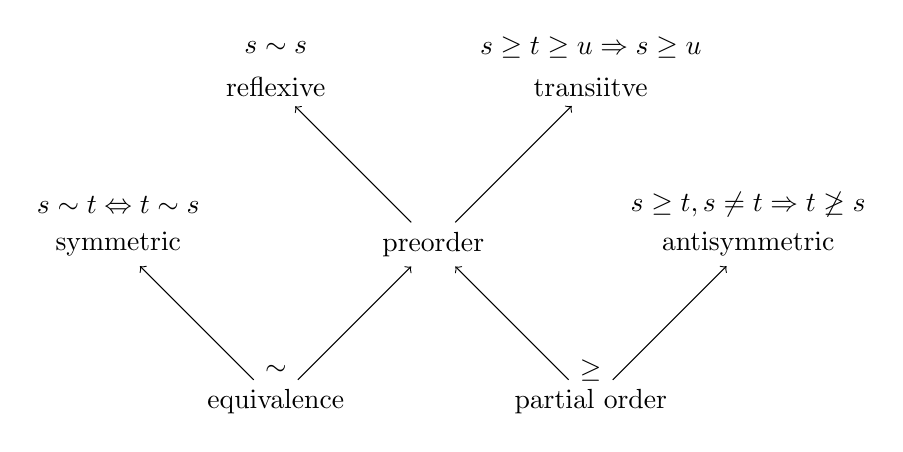
\begin{tikzpicture}
    \node (defREFLEXIVE) at (-2,2.5) { $s\sim s$ };
    \node (REFLEXIVE) at (-2,2) { reflexive };

    \node (defTRANSITIVE) at (2,2.5) { $s\geq t\geq u\Rightarrow s\geq u$ };
    \node (TRANSITIVE) at (2,2) { transiitve };

    \node (defTRANSITIVE) at (-4,0.5) { $s\sim t\Leftrightarrow t\sim s$ };
    \node (SYMMETRIC) at (-4,0) { symmetric };
    \node (PREORDER) at (0,0) { preorder };

    \node (defANTISYMMETRIC) at (4,0.5) { $s\geq t, s\neq t \Rightarrow t\not\geq s$ };
    \node (ANTISYMMETRIC) at (4,0) { antisymmetric };
    \node (SIM) at (-2,-1.6) { $\sim$ };
    \node (EQUIVALENCE) at (-2,-2) { equivalence };
    \node (GEQ) at (2,-1.6) { $\geq$ };
    \node (PARTIAL) at (2,-2) { partial order };

    \draw[->] (PREORDER) -- (REFLEXIVE);
    \draw[->] (PREORDER) -- (TRANSITIVE);

    \draw[->] (EQUIVALENCE) -- (SYMMETRIC);
    \draw[->] (EQUIVALENCE) -- (PREORDER);
    \draw[->] (PARTIAL) -- (PREORDER);
    \draw[->] (PARTIAL) -- (ANTISYMMETRIC);
\end{tikzpicture}
\caption{Equivalence relation vs.~partial order}
\end{center}
\end{figure}

\end{document}

\begin{document}

\begin{figure}
    \begin{center}
\begin{tikzpicture}
    \node (defCUC) at (-4,8.5) { \( s\succ t\Rightarrow \ctx[s]\succ \ctx[t] \)};
    \node (CUC) at (-4,8) { contexts };
    \node (defCUS) at (0,8.5) { \( s\succ t\Rightarrow s\sigma\succ t\sigma \)};
    \node (CUS) at (0,8) { substitutions };

    \node (ASYM) at (4,8.5) { \( s\succ t\Rightarrow t\not\succ s \) };
    \node (ASYM) at (4,8) { asymmetric };

        \node (CL) at (-2,6) { closed under };
        \node (defIRR) at (2,6.5) { \( s\succ t\succ u\Rightarrow s\succ u \) };
        \node (IRR) at (6,6) { irreflexive };
        \node (defIRR) at (6,6.5) { \( s\nsucc s \) };
        \node (TRA) at (2,6) { transitive };

        \node (POx) at (4,4.4) { \( > \) };
        \node (PO) at (4,4) { proper order };
        \node (RWRx) at (0,4.4) { \( \rightarrow^*_\mcR \) };
        \node (RWR) at (0,4) { rewrite relation };

        \node (defSTP) at (-2,2.5) { \( \ctx\neq\ctxhole\Rightarrow \ctx[s]\succ s \) };
        \node (STP) at (-2,2) { subterm property };
        \node (RWO) at (2,2) { rewrite order };
        \node (defWF) at (8,4.5) { \( \nexists s_0(s_i\succ s_{i+1})_{i=0}^{\infty} \) };
        \node (WF) at (8,4) { well-founded };

        \node (SO) at (0,0) {simplification order};
        \node (RO) at (4,0) {reduction order};

        \node (WFO) at (6,2) { well-founded order };


        \draw[->] (CL) -- (CUC);
        \draw[->] (CL) -- (CUS);

        \draw[->] (PO) -- (IRR);
        \draw[->] (PO) -- (TRA);

        \draw[->] (RWR) -- (CL);

        \draw[->] (RWO) -- (PO);
        \draw[->] (RWO) -- (RWR);

        \draw[->] (SO) -- (STP);
        \draw[->] (RO) -- (RWO);
        \draw[->] (RO) -- (WFO);
        % \draw (RO) edge[out=0,in=-45,->] (WF);

        \draw[->] (SO) -- (RWO);
        \draw[->, dotted] (SO) -- (RO);

        \draw[->] (WFO) -- (WF);
        \draw[->] (WFO) -- (PO);

        \draw[->, dotted] (WF) -- (IRR);

        % \node (TRAIRR) at (4,7) { \( \bullet \) };
        \draw[->, dotted] (4,7) -- (ASYM);

        \draw[dotted] (TRA) edge [out=-10, in=-90] (4,7);
        \draw[dotted] (IRR) edge [out=190, in=-90] (4,7);

        \draw[->, dotted] (ASYM) -- (IRR);
        % \draw[->, dotted] (ASYM) edge [out=0, in=0] (IRR);


    \end{tikzpicture}
\caption{Proper orders on terms}
    \end{center}
\end{figure}

\begin{figure}
    \begin{center}
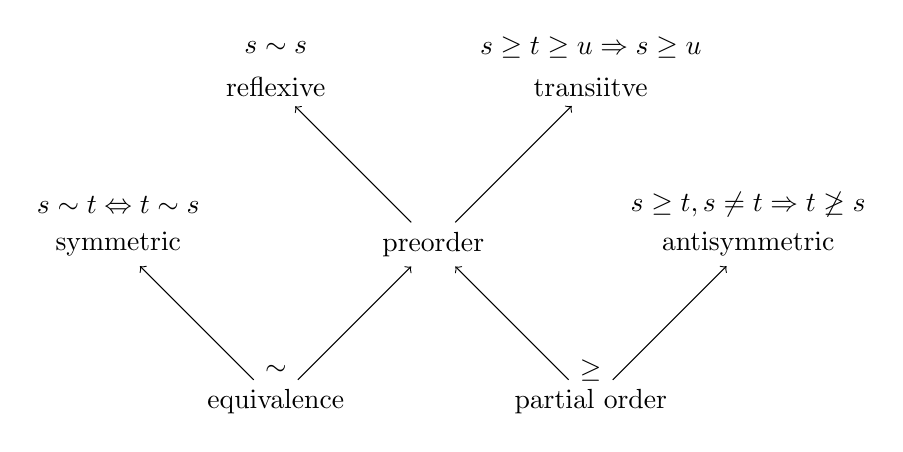
\begin{tikzpicture}
    \node (defREFLEXIVE) at (-2,2.5) { $s\sim s$ };
    \node (REFLEXIVE) at (-2,2) { reflexive };

    \node (defTRANSITIVE) at (2,2.5) { $s\geq t\geq u\Rightarrow s\geq u$ };
    \node (TRANSITIVE) at (2,2) { transiitve };

    \node (defTRANSITIVE) at (-4,0.5) { $s\sim t\Leftrightarrow t\sim s$ };
    \node (SYMMETRIC) at (-4,0) { symmetric };
    \node (PREORDER) at (0,0) { preorder };

    \node (defANTISYMMETRIC) at (4,0.5) { $s\geq t, s\neq t \Rightarrow t\not\geq s$ };
    \node (ANTISYMMETRIC) at (4,0) { antisymmetric };
    \node (SIM) at (-2,-1.6) { $\sim$ };
    \node (EQUIVALENCE) at (-2,-2) { equivalence };
    \node (GEQ) at (2,-1.6) { $\geq$ };
    \node (PARTIAL) at (2,-2) { partial order };

    \draw[->] (PREORDER) -- (REFLEXIVE);
    \draw[->] (PREORDER) -- (TRANSITIVE);

    \draw[->] (EQUIVALENCE) -- (SYMMETRIC);
    \draw[->] (EQUIVALENCE) -- (PREORDER);
    \draw[->] (PARTIAL) -- (PREORDER);
    \draw[->] (PARTIAL) -- (ANTISYMMETRIC);
\end{tikzpicture}
\caption{Equivalence relation vs.~partial order}
\end{center}
\end{figure}

\end{document}		% definitions and tikz macros
% \usepackage[thinlines,thiklines]{easybmat}
% %% ---------------------------------------------------------------------- %%

% %% -- Macros ------------------------------------------------------------ %%
% %% https://en.wikibooks.org/wiki/LaTeX/Macros
% \usepackage{xspace}
% !TeX encoding = UTF-8

%% ==============================================================
%% ### MY MATH ENVIRONMENTS ###

\theoremstyle{plain}
%\newtheorem{theorem}{Theorem}			% predefined in CL?
%\newtheorem{proposition}{Proposition}	% predefined in CL?
%\newtheorem{lemma}{Lemma}				% predefined in CL?
%\newtheorem*{corollary}{Corollary}		% predefined in CL?

\theoremstyle{definition}
%\newtheorem{definition}{Definition}	% predefined in CL?
\newtheorem{conjecture}{Conjecture}
%\newtheorem*{example}{Example}			% predefined in CL?
%\newtheorem{algorithm}{Algorithm}		% predefined in CL
\newtheorem{procedure}{Procedure}
\newtheorem{goal}{Goal}
\newtheorem{notation}{Notation}

\theoremstyle{remark}
\newtheorem*{remark}{Remark}			% predefined in CL?
\newtheorem*{observation}{Observation}
%\newtheorem*{note}{Note}
%\newtheorem{case}{Case}

%% ==============================================================
%% ### MY MATH DEFINITIONS ###

% math alphabets

\DeclareMathAlphabet{\mathpzc}{OT1}{pzc}{m}{it}	% \mathpzc
\DeclareMathAlphabet{\mathcll}{T1}{calligra}{m}{n}

% math operators

\DeclareMathOperator{\arity}{arity}		% arity of a symbol

\DeclareMathOperator{\var}{\mathpzc{Vars}}			% variables of a term
\DeclareMathOperator{\fun}{\mathpzc{Funs}}			% function symbols of a term
\DeclareMathOperator{\pos}{\mathpzc{Pos}}			% positions in a term
\DeclareMathOperator{\posT}{\mathpzc{{t-}Pos}}			% positions in a term
\DeclareMathOperator{\posS}{\mathpzc{Pos^F}}
%\DeclareMathOperator{\pos}{\mathcal{P}\mathsf{os}}
\DeclareMathOperator{\fvar}{\mathpzc{Fvars}}
\DeclareMathOperator{\bvar}{\mathpzc{Bvars}}

%\DeclareMathOperator{\var}{\mcV}			% variables of a term
%\DeclareMathOperator{\fun}{\mcFf}			% function symbols of a term
%\DeclareMathOperator{\pos}{\mathcal{P}\mathsf{os}}			% positions in a term

%\DeclareMathOperator{\T}{T}
	\DeclareMathOperator{\domain}{dom}			% domain of an assignment
	\DeclareMathOperator{\range}{rng}		% range of an assignment
	\DeclareMathOperator{\image}{img}			% image of an assignment
\DeclareMathOperator{\mgu}{mgu}			% most general unifier
%\DeclareMathOperator{\wgt}{W\!}
\DeclareMathOperator{\sel}{sel}			% selection function
%\DeclareMathOperator{\mul}{mul}
%\DeclareMathOperator{\add}{add}
\DeclareMathOperator{\head}{head}
\DeclareMathOperator{\tail}{tail}
\DeclareMathOperator{\length}{length}


%\DeclareMathOperator{\UNIF}{unifiable}
%\DeclareMathOperator{\INST}{instance}
%\DeclareMathOperator{\GNRL}{generalization}
%\DeclareMathOperator{\VRNT}{variant}
%\DeclareMathOperator{\PSTR}{pstr}

\DeclareMathOperator{\subterms}{\mathpzc{Subterms}}	
\DeclareMathOperator{\termsize}{size}
\DeclareMathOperator{\symbols}{symbols}
\DeclareMathOperator{\subforms}{\mathpzc{Subforms}}	
% !TeX encoding = UTF-8

% shortens the definition by cases
\newcommand{\DEFINE}[3][=]{{
		\begin{gather*}
		#2 #1 \left \{
				\begin{array}{ll}
					#3
				\end{array}
		\right.
		\end{gather*}
	}}

\newcommand{\MDEFINE}[4][=]{\ensuremath{
		#2 #1 \left \{
				\begin{array}{#3}
					#4
				\end{array}
		\right.
	}}


% accepts greek as input
\newcommand{\textgreek}[1]{\begingroup\fontencoding{LGR}\selectfont#1\endgroup}

\newcommand{\tikzmark}[1]{\tikz[overlay,remember picture] \node(#1) {};}


		% complex macros
% !TeX root = ../mythesis.tex
% !TeX encoding = UTF-8

% cspell:disable

%% ==============================================================
%% ### MISC ###



%% ==============================================================
% ### provide commands
%% ==============================================================
\providecommand{\colEm}{}	% not color et all
%% ==============================================================

% math alphabets

\DeclareMathAlphabet{\mathpzc}{OT1}{pzc}{m}{it}	% \mathpzc
\DeclareMathAlphabet{\mathcll}{T1}{calligra}{m}{n}

% math operators

\DeclareMathOperator{\arity}{arity}		% arity of a symbol

\DeclareMathOperator{\var}{\mathpzc{Vars}}			% variables of a term
\DeclareMathOperator{\fun}{\mathpzc{Funs}}			% function symbols of a term
\DeclareMathOperator{\pos}{\mathpzc{Pos}}			% positions in a term
\DeclareMathOperator{\posT}{\mathpzc{{t-}Pos}}			% positions in a term
\DeclareMathOperator{\PosStr}{\mathpzc{Pos^F}}
\DeclareMathOperator{\vaPosStr}{\mathpzc{Pos^F_*}}
\DeclareMathOperator{\posV}{\mathpzc{Pos^{\!V}}}
\DeclareMathOperator{\occurs}{occurs}
\DeclareMathOperator{\fvar}{\mathpzc{Fvars}}
\DeclareMathOperator{\bvar}{\mathpzc{Bvars}}

\DeclareMathOperator{\domain}{dom}			% domain of an assignment
\DeclareMathOperator{\range}{rng}		% range of an assignment
\DeclareMathOperator{\image}{img}			% image of an assignment
\DeclareMathOperator{\IRRED}{irred}

\DeclareMathOperator{\mgu}{mgu}			% most general unifier
\DeclareMathOperator{\sel}{sel}			% selection function

%\DeclareMathOperator{\mul}{mul}
%\DeclareMathOperator{\add}{add}
\DeclareMathOperator{\head}{head}
\DeclareMathOperator{\tail}{tail}
\DeclareMathOperator{\length}{length}

\DeclareMathOperator{\UNIF}{unifiable}
\DeclareMathOperator{\INST}{instance}
\DeclareMathOperator{\GNRL}{generalization}
\DeclareMathOperator{\VRNT}{variant}
\DeclareMathOperator{\SUBS}{subsumses}
\DeclareMathOperator{\PSSTR}{substring}
\DeclareMathOperator{\PSTR}{pstr}

%\DeclareMathOperator{\subterms}{\mathpzc{Subterms}}
%\DeclareMathOperator{\termsize}{size}
%\DeclareMathOperator{\symbols}{symbols}
%\DeclareMathOperator{\subforms}{\mathpzc{Subforms}}


%\newcommand\TOP[2]{\genfrac{}{}{0pt}{}{#1}{#2}}
%\newcommand\TOPTEXT[2]{\TOP{\text{#1}}{\text{#2}}}
%\newcommand{\mygreek}[1]{\selectlanguage{polutonikogreek}#1\selectlanguage{english}}
%\newcommand{\mygreek}[1]{{\selectlanguage{polutonikogreek}#1}\selectlanguage{english}}
%\renewcommand{\mygreek}[1]{\foreignlanguage{polutonikogreek}{#1}}

%\newcommand{\iSUB}[2]{#2\!\mapsto\!#1}
%\newcommand{\BgSyntaxTree}{\usebackgroundtemplate{\transparent{0.1}\includegraphics[width=\paperwidth]{SyntaxTreeBackground.png}}}

%\newcommand{\EMPH}[1]{\emph{\textcolor{colEm}{#1}}}
\newcommand{\coloremph}[1]{\textcolor{colEm}{\emph{#1}}}


%\newcommand{\NGTPREQ}{\not\succcurlyeq}

\newcommand{\succG}{\mathrel\succ_{\!\mathtt{gr}}}
\newcommand{\succL}{\mathrel\succ_{\mathtt{L}}}
\newcommand{\succC}{\mathrel\succ_{\mathtt{C}}}

\newcommand{\disjointunion}{\mathbin{\dot\cup}}
\newcommand{\limp}{\rightarrow}		% logical implication, see lor, land, lnot
\newcommand{\lbic}{\leftrightarrow} % logical biconditional

% constant (function, predicate) symbols

\newcommand{\true}{\mathsf{true}}
\newcommand{\false}{\mathsf{false}}

\newcommand{\ma}{\mathsf{a}}
\newcommand{\mb}{\mathsf{b}}
\newcommand{\mc}{\mathsf{c}}
\newcommand{\md}{\mathsf{d}}
\newcommand{\me}{\mathsf{e}}
\newcommand{\mf}{\mathsf{f}}
\newcommand{\mg}{\mathsf{g}}
\newcommand{\mh}{\mathsf{h}}

\newcommand{\mA}{\mathsf{A}}
\newcommand{\mB}{\mathsf{B}}
\newcommand{\mE}{\mathsf{E}}
\newcommand{\mL}{\mathsf{L}}
\newcommand{\mN}{\mathsf{N}}
\newcommand{\mP}{\mathsf{P}}
\newcommand{\mQ}{\mathsf{Q}}
\newcommand{\mR}{\mathsf{R}}

\newcommand{\mpp}{\mathsf{p}}
\newcommand{\mpq}{\mathsf{q}}

\newcommand{\msucc}{\mathsf{s}}
\newcommand{\mpred}{\mathsf{p}}
\newcommand{\mzero}{\mathsf{z}}

\newcommand{\mEQ}{\approx}			% \simeq
\newcommand{\mNE}{\not\approx}		% \not\simeq

%\newcommand{\rwEQ}{\rightarrow}			% rewrite equation
\newcommand{\rwStep}[1][]{\xrightarrow[{}]{#1}}	% rewrite step

\newcommand{\defEQ}[1][def]{\stackrel{\text{#1}}{=}}
\newcommand{\defEV}[1][def]{\stackrel{\text{#1}}{\equiv}}

%\newcommand{\dis}{{\wr}}
\newcommand{\encsep}{\cdot} % encoding separator
\newcommand{\pthsep}{.} % path separator

% general terms or symbols

\newcommand{\mkf}{\mathfrak{f}}
\newcommand{\mkg}{\mathfrak{g}}
\newcommand{\mkr}{\mathfrak{r}}
\newcommand{\mks}{\mathfrak{s}}
\newcommand{\mkt}{\mathfrak{t}}

% calligraphic symbol

\newcommand{\mcA}{\mathcal{A}}
\newcommand{\mcB}{\mathcal{B}}
\newcommand{\mcC}{\mathcal{C}}
\newcommand{\mcD}{\mathcal{D}}
\newcommand{\mcE}{\mathcal{E}}
\newcommand{\mcF}{\mathcal{F}}	% signature
\newcommand{\mcG}{\mathcal{G}}
\newcommand{\mcH}{\mathcal{H}}
\newcommand{\mcI}{\mathcal{I}}
\newcommand{\mcL}{\mathcal{L}}
\newcommand{\mcM}{\mathcal{M}}
\newcommand{\mcN}{\mathcal{N}}
\newcommand{\mcO}{\mathcal{O}}
\newcommand{\mcP}{\mathcal{P}}
\newcommand{\mcR}{\mathcal{R}}
\newcommand{\mcS}{\mathcal{S}}
\newcommand{\mcT}{\mathcal{T}}
\newcommand{\mcV}{\mathcal{V}}
\newcommand{\mcX}{\mathcal{X}}

\newcommand{\mca}{\mathpzc{a}}
\newcommand{\mcb}{\mathpzc{b}}
\newcommand{\mcc}{\mathpzc{c}}
\newcommand{\mce}{\mathpzc{e}}
\newcommand{\mcf}{\mathpzc{f}}
\newcommand{\mcg}{\mathpzc{g}}
\newcommand{\mch}{\mathpzc{h}}
\newcommand{\mcp}{\mathpzc{p}}
\newcommand{\mcq}{\mathpzc{p}}
\newcommand{\mcr}{\mathpzc{r}}
\newcommand{\mcs}{\mathpzc{s}}
\newcommand{\mct}{\mathpzc{t}}
\newcommand{\mcu}{\mathpzc{u}}

\newcommand{\mysymbol}{\mcf}

% signature, terms, predicates, equations

\newcommand{\mcFf}{{\mcF_\mf}}		% function symbols
\newcommand{\mcFP}{{\mcF_\mP}}		% predicate symbols
\newcommand{\mcCon}{\mcF_\mathsf{con}}
\newcommand{\mcAux}{\mcF_\mathsf{aux}}
\newcommand{\mcFfPE}{\ensuremath{\mcFf \disjointunion \mcFP \disjointunion \{\mEQ \}}}

\newcommand{\mcTf}{\mcT_\mf}						% terms (short)
\newcommand{\mcTFf}{{\mcT(\mcF_\mf,\emptyset)}}		% ground terms (long)
\newcommand{\mcTFfV}{{\mcT(\mcF_\mf,\mcV)}}		% terms (long)
\newcommand{\mcPT}{\mcP(\mcFP,\mcTf)}				% predicates
\newcommand{\mcET}{\mcE(\mEQ, \mcTf)}				% equations


\newcommand{\mNF}[1]{\mathsf{NF} (#1)}	% Normal Form
\newcommand{\mNFR}{\mNF{\mcR}}		% set of normal forms

% reevaluate:
\newcommand{\mcFn}[1][n]{\mcF^{(#1)}}
\newcommand{\mcFfn}[1][n]{{\mcFn[#1]_\mf}}
\newcommand{\mcFPn}[1][n]{{\mcFn[#1]_\mP}}

\newcommand{\vecn}[1]{\vec{#1}}


% terms with signature
% \newcommand{\mcTFV}{{\mcT(\mcFf,\!\mcV)}}
%\newcommand{\mcTFV}{{\mcT(\mcF\!,\mcV)}}		% the set of function terms


%\newcommand{\Var}{{}\mcV\mathsf{ar}}
%\newcommand{\Dom}{{}\mcD\mathsf{om}}
%\newcommand{\Pos}{{}\mcP\mathsf{os}}
%\newcommand{\PosStr}{\Pos^\Sigma}

% fraktal symbols

\newcommand{\mfC}{\mathfrak{C}}
\newcommand{\mfL}{\mathfrak{L}}
\newcommand{\mfR}{\mathfrak{R}}
\newcommand{\mfT}{\mathfrak{T}}

\newcommand{\SIGA}{\mathcal{A}}
\newcommand{\SIGC}{\mathcal{C}}
\newcommand{\SIGE}{\mathcal{E}}
\newcommand{\SIGF}{\mathcal{F}}
\newcommand{\SIGL}{\mathcal{L}}
\newcommand{\SIGP}{\mathcal{P}}
\newcommand{\SIGS}{\mathcal{S}}
\newcommand{\SIGT}{\mathcal{T}}
\newcommand{\SIGV}{\mathcal{V}}
% tt symbols

\newcommand{\mtS}{\mathtt{S}}
\newcommand{\sgr}{\succ_{\mathsf{gr}}}

%

% first order expression)
\newcommand{\foxf}{\textcolor{colO}{\mcf}} % predicate or function symbol f
\newcommand{\foxt}{\textcolor{colO}{\mct}} % atom or term t
\newcommand{\foxs}{\textcolor{colO}{\mcs}} % atom or term t


\newcommand{\TI}[1]{^{^{#1:}}\!}
\newcommand{\ANGLES}[1]{\langle#1\rangle}

\newcommand{\joins}{\rightarrow^*\cdot^*\! \!\leftarrow}
\newcommand{\meets}{\ensuremath{^*\! \!\leftarrow \cdot \rightarrow^* }}


\newcommand{\mCP}[1]{\mathsf{CP} (#1)}		% Critical Pair
\newcommand{\mCPR}{\mCP{\mcR}}		% CP(R)

\newcommand{\MUL}[2]	% multiplication
{\mf(#1,#2)}			% mul(x,y)
%{#1\cdot #2}			% x.y

\newcommand{\ADD}[2]	% addition
{\add(#1,#2)}			% add(x,y)
%{#1+#2}				% x+y

\newcommand{\MYPOS}[1]{\ensuremath{\tt #1}}
\newcommand{\overlap}[3]{\ensuremath{\langle #1,\MYPOS{#2}, #3 \rangle}}
\newcommand{\overlapN}[4]{\ensuremath{_{\overlap{#1}{#2}{#3}}}^{#4:\;}}

%\newcommand{\GTKBO}{>_{\tt kbo}}
\newcommand{\GTKBOW}[2]{\texttt{SMT} (#1\!>_\texttt{kbo}\!#2)}
\newcommand{\GTKBOP}[2]{\texttt{SMT} (#1\!>_\texttt{kbo}'\!#2)}

\newcommand{\UPL}{\ensuremath{\infer[(\sigma)
		\quad\sigma=\mgu(l,l'), l'\!\not\in\mcV, l\sigma\rho\sgr r\sigma\rho
	]
	{L[r]\sigma}
	{l=r & L[l']}}
}

\newcommand{\ctxhole}{\square} %{\boxdot}
\newcommand{\ctx}[1][\ ]{\mathtt{C[}#1\mathtt{]}} % chktex 9
\newcommand{\emptyclause}{\square}
\newcommand\relation{\mathrel{\circledast}}	% \currency

\usepackage{pifont}% http://ctan.org/pkg/pifont

\newcommand{\cmark}{\ding{51}}
\newcommand{\xmark}{\ding{55}}

\newcommand{\species}{\mathsf{species}}
\newcommand{\human}{\mathsf{human}}
\newcommand{\mortal}{\mathsf{mortal}}
\newcommand{\socrates}{\mathsf{socrates}}
\newcommand{\fosca}{\mathsf{fosca}}

\newcommand{\ack}{\mathsf{ack}}

\newcommand{\InstGen}{\texttt{Inst-Gen}\xspace}
\newcommand{\InstGenEQ}{\texttt{Inst-Gen-Eq}\xspace}
\newcommand{\SAT}[1][\xspace]{\texttt{SAT}#1}
\newcommand{\UNSAT}[1][\xspace]{\lnot\SAT[#1]}
\newcommand{\SMT}[1][\xspace]{\texttt{SMT}#1}


\newcommand{\consbot}{\ensuremath{\mc \!_\bot}}	% Inst-Gen bot, i.e. distinct constant symbol not in the signature
\newcommand{\subsbot}{\ensuremath{\sigma \!_\bot}}

\newcommand{\CNF}{\texttt{CNF}\xspace}
\newcommand{\FOF}{\texttt{FOF}\xspace}
\newcommand{\PNF}{\texttt{PNF}\xspace}
\newcommand{\FLEA}{\texttt{FLEA}\xspace}
\newcommand{\TPTP}{\texttt{TPTP}\xspace}
\newcommand{\TPTPtgz}{\texttt{TPTP-v7.1.0.tgz}\xspace}
\newcommand{\GitHubInc}{\texttt{GitHub,\;Inc.}\xspace}
\newcommand{\GitHub}{\texttt{GitHub}\xspace}
\newcommand{\Swift}{\texttt{Swift\;4.1}\xspace}
\newcommand{\Yices}{\texttt{Yices\;2}\xspace}
\newcommand{\Ziii}{\texttt{Z3}\xspace}

% \newcommand{\landlor}{\mathrel{\ooalign{\hss\( \land \)\hss\cr\( \lor \)}}}
%\newcommand{\limpxor}{\mathrel{\ooalign{\hss\( \limp \)\hss\cr\( \oplus \)}}}
\newcommand{\quantify}{{\rotatebox[origin=c]{180}{\textsf{\AE}}}\!}
%\newcommand{\junction}{\landlor}
% \newcommand{\logical}{\mathrel{\ooalign{\hss\( \landlor \)\hss\cr\( \limp \)}}}

\newcommand{\prompt}{\$}
\newcommand{\proves}{\vdash}

\newcommand{\entails}{\vDash}
\newcommand{\equival}{\equiv}
\newcommand{\equisat}{%
	\mathrel{\vcenter{\offinterlineskip{}
			\hbox{\( \sim \)}\vskip-.35ex\hbox{\( \sim \)}\vskip-.35ex\hbox{\( \sim \)}}}} % chktex 41


%\newcommand{\jek}{(\Lightning?)}
% \newcommand{\jek}{(\Lightning{}\( _\true^? \))}
\newcommand{\jek}{(\Lightning{}\( ^? \))}

\newcommand{\MAXIMAL}[1]{\boxed{\color{colMAXIMAL}#1}}
\newcommand{\STRICTLY}[1]{\boxed{\color{colSTRICTLY}#1}}

\newcommand{\txtMAXIMAL}{\textcolor{colMAXIMAL}{maximal}\xspace}
\newcommand{\txtSTRICTLY}{\textcolor{colSTRICTLY}{strictly maximal}\xspace}

\newcommand{\MISSING}[1]{\texttt{--MISSING>> #1 <<MISSING--}}
\newcommand{\IMPROVE}[1]{\texttt{--IMPROVE>> #1 <<IMPROVE--}}
\newcommand{\OBSOLETE}[1]{\texttt{--OBSOLETE>> #1 <<OBSOLETE--}}




			% simple macros
% %% ---------------------------------------------------------------------- %%

% \usepackage{epigraph}

